\documentclass[11pt]{article}
\usepackage[review]{acl}
\usepackage{times}
\usepackage{latexsym}
\usepackage[T1]{fontenc}
\usepackage[utf8]{inputenc}
\usepackage{microtype}
\usepackage{inconsolata}
\usepackage{graphicx}
\usepackage{booktabs}
\usepackage{amsmath,amssymb,amsthm}
\usepackage{xcolor}
\newtheorem{proposition}{Proposition}
\newcommand{\eps}{\varepsilon}
\newcommand{\HES}{\mathrm{HES}}
\newcommand{\Jt}{J_{50}}

\title{From System Ranking to Decision Value:\\ How Much Human Evaluation Do Automatic Evaluators Actually Save?}

\author{Anonymous ACL submission}

\begin{document}
\maketitle

\begin{abstract}
Automatic evaluators, from learned metrics to LLM judges, are increasingly credited with the human labels they save, and
that credit is usually inferred from their correlation with human scores. We measure it directly for a concrete decision:
certifying, from a human audit, that a selected system is within $\eps$ of the best of a menu of close competitors. An
evaluator's human-evidence saving (HES) is the fraction of human labels, pilot included, that it saves for this decision
over the best fixed annotation design that uses no evaluator. Across machine translation (WMT22 MQM; 31 segment-level
metric variants and open LLM judges), chat (LMArena) and retrieval, with prospectively locked MT and chat evaluations,
evaluator quality turns out to depend on the level at which it is measured: metrics with system-level correlations of
0.93--0.99 reach correlations of only 0.11--0.38 on the paired differences a close decision depends on. Correspondingly,
the eleven strongest evaluators save on average 0--7\% of human labels on top of a judge-free design, even when the
correction coefficient is refitted on all labels as in standard PPI++, while the judge-free design itself, mostly by not
re-rating identical outputs, saves 8--16\% in MT and 41--56\% in retrieval. Fixing the coefficient on a 50-item pilot
before the audit costs a further 2.5--4.3 points, which refitting removes and cross-fitting only partly recovers.
\end{abstract}

\section{Introduction}
Human judgments remain the reference for comparing NLP systems, and they are expensive. Automatic evaluators promise to
stretch them: score everything automatically and spend human effort only on correcting the evaluator's bias, as in
prediction-powered inference \citep[PPI;][]{angelopoulos2023ppi,angelopoulos2023ppipp}. How much an evaluator saves
under such a correction is now measured directly \citep{boyeau2024autoeval,chen2026noisy}, and \citet{gao2026ppsr}
propose to rank MT metrics by the annotation they save (PPSR), which is governed by the squared correlation between
human and metric score \emph{differences}.

We ask what that saving amounts to for the decision an evaluation is usually run for. A team has a short list of strong
systems that are close in quality, and wants to certify from a human audit that the one it picks is within $\eps$ of the
best. Three things separate this setting from the asymptotic picture. First, the decision is local: the systems that
matter are the top few, not the whole field over which system-level correlation is computed. Second, a human audit need
not sample uniformly: items whose paired difference is known to be zero (identical outputs, documents outside every
system's cutoff) need no label, and others can be sampled in proportion to how much they can move the decision. Third,
the coefficient that corrects the evaluator must itself be estimated from the few human labels the audit has.

\paragraph{Contributions.}
\begin{enumerate}
\item \textbf{A decision-level measure of evaluator value.} The human-evidence saving
$\HES=1-\Jt(\text{design}+\text{evaluator})/\Jt(\text{best fixed judge-free design})$, with $\Jt$ the number of unique
human labels, pilot included, at which the decision is certified with probability $1/2$ (\S\ref{sec:setup}).
\item \textbf{Evaluator quality collapses across levels.} On WMT22 en$\to$de and zh$\to$en, metric variants with system-level
Pearson 0.93--0.99 rank the top-4 zh$\to$en systems in exactly reversed order for 10 of 31 variants, reach decision-level
correlations of 0.11--0.38, and realise HES between $-10\%$ and $+7\%$ (\S\ref{sec:levels}).
\item \textbf{A judge-free design saves more than the typical evaluator.} In all four pre-registered MT cells the
design saves more than the best of 31 metric variants adds on top of it with a pilot-fixed coefficient (8--16\% vs.\
$\le 7\%$), and more than the mean of the eleven strongest evaluators under every coefficient rule we tried; the best
evaluator chosen post hoc exceeds it in two of four cells when the coefficient is refitted. Retrieval: 41--56\% of
uniform-sampling labels vs.\ 1--9 further points (\S\ref{sec:design}).
\item \textbf{Committing to the coefficient early has a price.} Fitting the correction on a 50-item pilot costs 4.3 [3.5,
5.2] (en$\to$de) and 2.5 [2.0, 3.1] (zh$\to$en) points over the 31 variants; refitting on all labels removes this tax with
no detected loss of calibration in our simulations, and cross-fitting recovers it on zh$\to$en but not on en$\to$de
(\S\ref{sec:law}).
\item \textbf{Pre-registered, with failures reported.} Four locks fixed hypotheses before the corresponding evaluator
outputs were joined with human labels; of the ten hypotheses tested, H2, H5 and H6 failed and H4 failed in chat; all are reported with their explanations (\S\ref{sec:prereg}).
\end{enumerate}
We propose no estimator: the corrected estimator is PPI++ with a pilot-fixed coefficient, and the allocation is
active statistical inference \citep{zrnic2024active} for the decision's functional.

\section{Setup}\label{sec:setup}
\paragraph{Decision.} A menu $\mathcal M$ of systems is evaluated on a fixed set of $N$ items with human utilities
$u_m(i)$ and means $\mu_m$. An audit labels a pilot of $P$ items fully, picks the candidate $\hat m$ with the best pilot
mean, and \emph{certifies} it if for every competitor $j$ a one-sided upper bound on $\mu_j-\mu_{\hat m}$ is at most
$\eps$ (normal bound, Bonferroni over competitors, $\alpha=0.10$). A certificate is wrong if
$\max_j\mu_j-\mu_{\hat m}>\eps$. Menus are deliberately hard: we use the full human labels only to construct them
(the top-4 systems by human MQM, or the closest Arena pairs); menu construction is not part of the audit.

\paragraph{Estimator.} After the pilot, items are drawn by Poisson sampling with probabilities $\pi_i$. For
$D_j=u_j-u_{\hat m}$ and an evaluator's predicted difference $\hat D_j$,
\begin{equation}
\hat\Delta_j=\tfrac1N\Big[\sum_{\text{pilot}}D_j+\sum_{\text{rest}}\lambda_j\hat D_j+\sum_{i\in S}\tfrac{D_j(i)-\lambda_j\hat D_j(i)}{\pi_i}\Big],\label{eq:est}
\end{equation}
with $\lambda_j=\max(0,\widehat{\mathrm{Cov}}(D_j,\hat D_j)/\widehat{\mathrm{Var}}(\hat D_j))$ fitted on the pilot and
frozen; $\lambda=0$ is the human-only estimator. Given the pilot, (\ref{eq:est}) is unbiased for the finite-population
mean for any evaluator; its variance is estimated by $\sum_S(1-\pi_i)R_i^2/(\pi_i^2N^2)$, $R=D-\lambda\hat D$.

\paragraph{Designs.} \emph{Uniform}: constant $\pi$; every menu output of a sampled item is labelled, identical
strings included (the usual practice of rating each system's output). \emph{Dedup}: uniform over items where some
competitor's output differs from the candidate's, identical strings rated once, and $D_j=0$ used exactly where outputs
coincide. \emph{Weighted}: as dedup, with items sampled in proportion to a label-free proxy of $|D|$ (in retrieval the
closed-form decision weight of each document; in MT $\sqrt{\sum_j\hat\sigma^2_j(b)}$, with $\hat\sigma^2_j(b)$ the pilot
mean of $D_j^2$ in one of four quartile bins $b$ of the chrF-based dissimilarity of the two outputs). The \emph{best fixed judge-free baseline} of a cell is the cheapest
of these human-only designs there; it is a benchmark, not a procedure an auditor selects. An evaluator enters as the
control variate of (\ref{eq:est}) on top of a design.

\paragraph{Cost.} $\Jt$ counts unique human labels, pilot included, at which a pre-committed budget certifies in half of
300 simulated audits (linear interpolation over a geometric grid of 14 budgets). The 50-segment MT pilot costs 162
(en$\to$de) and 182 (zh$\to$en) labels, 42--68\% of $\Jt$ on en$\to$de; an evaluator can act only on the rest, which the
factor $1-P/J$ of \S\ref{sec:law} makes explicit. Intervals are paired bootstraps over the 300 simulated audits of a
fixed test set: they reflect Monte-Carlo, not data-sampling, uncertainty.

\section{Data, evaluators and protocol}\label{sec:data}
\textbf{MT:} WMT22 MQM \citep{freitag2021mqm} en$\to$de (1{,}315 segments) and zh$\to$en (1{,}875), Google weights,
$u=-\min(\mathrm{MQM},25)/25$, identical output strings of a segment share the mean of their ratings; menus of the four best WMT submissions
(MBR systems excluded). Evaluators: the 31 WMT22 metric variants available at segment level in mt-metrics-eval \citep{freitag2022wmt22metrics}
(reference-based variants scored against refA, including COMET-22 \citep{rei2022comet}, and reference-free QE variants),
plus our own COMET-22 run and Qwen3-8B \citep{yang2025qwen3} and Mistral-7B-Instruct-v0.3 \citep{jiang2023mistral} with the GEMBA-DA prompt \citep{kocmi2023gemba}.
\textbf{Chat:} LMArena human-preference battles \citep{chiang2024arena}; the six English single-turn pairs with the
smallest win-rate gaps among those with $\ge300$ battles (311--472 battles; gaps 0.011--0.084). Evaluators: Qwen3-8B and
Mistral-7B as pairwise judges (both presentation orders averaged), ``the longer response wins''.
\textbf{Retrieval:} a re-analysis of fixed-budget audits from an earlier study, in which three cutoff policies over a
shared ranked pool (an expected-F1 gate, a global score threshold and a learned truncation) are compared by precision
at their cutoffs, $\eps$ in precision units, on four fully judged collections
(ANTIQUE, CAsT 2019, DBpedia-Entity, TREC DL 21--23; \citealp{hashemi2020antique,dalton2020cast,hasibi2017dbpedia,craswell2021dl21,craswell2022dl22,craswell2023dl23}) with Qwen3-8B (UMBRELA prompt; \citealp{upadhyay2024umbrela}) and Qwen3-Reranker-0.6B \citep{zhang2025qwen3embedding} as judges; pilot
20 queries. MT and chat use a 50-item pilot (ablations: 100 for MT, 25 for chat), $\eps\in\{0.01,0.02\}$ (MT) and
$\{0.05,0.1\}$ (chat).

\paragraph{Pre-registration.} Lock v0.8 (MT, chat) was committed before any LLM or COMET judgment was joined with a human
label; v0.9 replaced the uninformative v0.8 chat decision (gaps 0.10--0.56 were settled by the pilot alone) by close
pairs before they were judged; v1.1 fixed the 31-metric test before any of its savings were computed; v1.0 (frontier
judges) is committed and not yet run. All locks were committed within one day on public data whose human labels
exist; before v0.8 the human-only MT designs had been run in development (they saved 8--19\% over
uniform sampling and chrF saved about nothing, so H1 was not a blind test), and v1.1 was written after the exploratory
estimation-tax and $\rho$-dial analyses of the open judges, so H9 tests on 31 new evaluators a phenomenon first seen
on four. The retrieval results are a re-analysis; their held-out test (NeuCLIRBench) followed a lock of the earlier
study that is not part of this repository. All locks, deviations and outcomes are in the supplementary material.

\section{Evaluator quality depends on the level of measurement}\label{sec:levels}
Figure~\ref{fig:levels} places the 30 positively correlated WMT22 metric variants (REUSE omitted) on three levels against their realised HES. At the global level
(Pearson over the 11 WMT submissions) nearly all strong metrics are above 0.9; this is the quantity metric shared tasks
report. Among the four closest systems the ranking is fragile: MetricX-XL-DA and MetricX-XXL-DA reach system-level
Pearson 0.994--0.995 on zh$\to$en and Kendall $\tau=0$ among the top four; BLEURT-20 reaches 0.980 and $\tau=-0.33$ (zh$\to$en). The second- and third-ranked systems differ by
only 0.0009 (en$\to$de) and 0.0017 (zh$\to$en) in utility (standard error 0.002--0.004), so $\tau=0$ can reflect fragility;
but 10 of the 31 zh$\to$en variants reach $\tau=-1$, reversing gaps that are resolved. The
quantity that governs a control variate is the correlation $\rho$ of per-item paired differences, and it is low
everywhere: 0.30--0.38 for the best metrics on en$\to$de (mean over the menu's pairs), 0.21--0.25 on zh$\to$en, and 0.17--0.29 for COMET-22 and the
Qwen3-8B GEMBA judge (system-level 0.97--0.99; here medians over pairs of the top-6 systems), while the Mistral-7B GEMBA
judge reaches only 0.04--0.09. Realised HES over the best judge-free baseline lies between $-10\%$ and $+7\%$ for
every metric and cell. Across metrics, HES is ranked slightly better by $\rho$ than by system-level Pearson (Spearman 0.39 vs.\
0.36 on en$\to$de, 0.22 vs.\ 0.07 on zh$\to$en; H11), but neither predicts it well among real metrics, because all of
them sit in the region where the saving is small (\S\ref{sec:law}).

\begin{figure*}[t]\centering
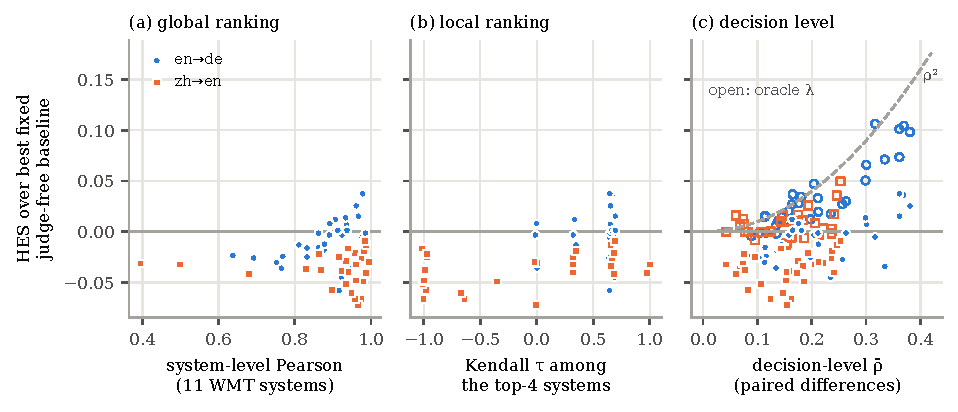
\includegraphics[width=\textwidth]{figures/F1_levels.pdf}
\caption{Thirty WMT22 metric variants at three levels of quality against their realised human-evidence saving over the best
fixed judge-free baseline (pilot 50, mean over $\eps\in\{0.01,0.02\}$). (c) open markers: the same metrics with the
population-optimal (oracle) correction coefficient; dashed: $\rho^2$, the asymptotic saving. REUSE (negative system-level
correlation; switched off by $\lambda\ge0$) is omitted.}\label{fig:levels}
\end{figure*}

\section{Where the savings come from}\label{sec:design}
Figure~\ref{fig:waterfall} and Table~\ref{tab:main} decompose the saving over uniform sampling into the part a judge-free design obtains and the
part the best evaluator adds on top. In retrieval, skipping documents that no comparison depends on and sampling the rest
by decision weight saves 41--56\% of the labels of uniform sampling; the Qwen3-8B judge adds 1--9 points of that total
(HES 3--20\% over the design). In MT, identical outputs (14--24\% of segment pairs in the en$\to$de menu, 5--16\% in zh$\to$en) need no label,
and many paired MQM differences are exactly zero (53--59\% and 40--48\%); exploiting this saves 16\% (en$\to$de) and 8\%
(zh$\to$en) at $\eps=0.01$. The best of the 31 metric variants, chosen \emph{post hoc} and therefore favoured, adds 7\% and
$-1\%$. In all four pre-registered MT cells the design's saving exceeds the best metric's increment (H8, 4/4; H1 with
the open judges, 4/4). Most of the MT design saving is deduplication: not re-rating identical outputs saves 13\% and
6\% on en$\to$de and all 8\% on zh$\to$en, where proxy-weighted sampling adds nothing.

In retrieval, the evaluator's increment follows its decision-level correlation as well: across 54 settings of an
earlier query-level study the realised gain correlated 0.75 with $\rho$ and 0.03 with label accuracy; an identical-model
judge over-credited its own policy by 0.14 F1, a bias the correction removes, while the noise that accompanied it lowered
$\rho$ and the saving. In a locked test on a collection never used in development (NeuCLIRBench; \citealp{lawrie2025neuclirbench}), a 20-query pilot
predicted the relative cost of designs (correlation 0.83--0.97) but over-estimated the judge's own increment
(predicted cost ratio 0.71--0.76, realised 0.82--0.93), the estimation-tax pattern of \S\ref{sec:law}.

\begin{figure}[t]\centering
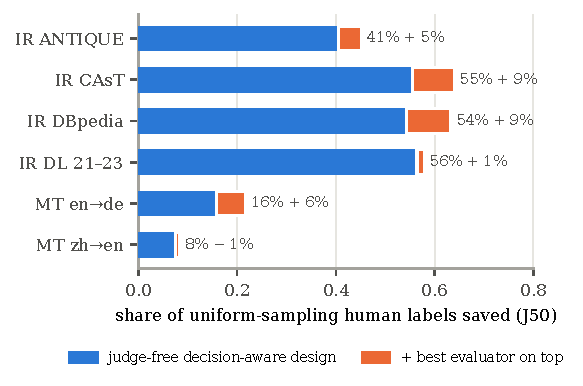
\includegraphics[width=\columnwidth]{figures/F2_waterfall.pdf}
\caption{Share of uniform-sampling human labels ($\Jt$) saved by the best fixed judge-free design and added by the best
evaluator on top, both as shares of uniform-sampling labels (retrieval: Qwen3-8B, $\eps=0.02$; MT: best of 31 metric
variants post hoc, pilot-fixed coefficient, $\eps=0.01$; e.g.\ en$\to$de's 6 points are a 7\% HES over the design).}\label{fig:waterfall}
\end{figure}

\begin{table}[t]\centering\footnotesize\setlength{\tabcolsep}{3pt}
\resizebox{\columnwidth}{!}{\begin{tabular}{lrrrr}\toprule
Cell & uniform & judge-free & + evaluator & evaluator\\
 & $\Jt$ & best fixed & best (median) & HES\\\midrule
IR ANTIQUE & 1{,}405 & 836 & 770 & 8\%\\
IR CAsT 2019 & 4{,}778 & 2{,}127 & 1{,}720 & 19\%\\
IR DBpedia-Entity & 5{,}563 & 2{,}543 & 2{,}046 & 20\%\\
IR DL 21--23 & 4{,}092 & 1{,}783 & 1{,}722 & 3\%\\\midrule
MT en$\to$de, $\eps$=.01 & 463 & 389 & 362 (390) & 7\% (0\%)\\
MT en$\to$de, $\eps$=.02 & 261 & 238 & 233 (242) & 2\% ($-2$\%)\\
MT zh$\to$en, $\eps$=.01 & 2{,}990 & 2{,}738 & 2{,}764 (2{,}838) & $-1$\% ($-4$\%)\\
MT zh$\to$en, $\eps$=.02 & 1{,}166 & 1{,}066 & 1{,}058 (1{,}100) & 1\% ($-3$\%)\\\bottomrule
\end{tabular}}
\caption{Unique human labels ($\Jt$, pilot included) for uniform sampling, the best fixed judge-free design, and that
design with an evaluator. Retrieval: Qwen3-8B judge, $\eps=0.02$, pilot 20 queries. MT: the best of the 31 WMT22 metric variants
chosen post hoc, and the median metric in parentheses; pilot 50 segments. MT evaluators are applied on the weighted
design; for zh$\to$en the best fixed judge-free design is dedup, and on that matched base the best of the 11 strongest
evaluators saves 7.3\% ($\eps=0.01$) and $-0.5\%$ ($\eps=0.02$), \S\ref{sec:law}.}\label{tab:main}
\end{table}

\section{From correlation potential to realised saving}\label{sec:law}
\begin{proposition}[Finite-pilot cost approximation]\label{prop:law}
Let a design need $L_0$ post-pilot labels for a fixed decision without an evaluator, and let the evaluator's paired
differences $\hat D$ have correlation $\rho$ with the human ones $D$. Assume that, over informative items (those with a
non-zero difference), $D$ is a linear projection on $\hat D$ with a residual whose variance does not depend on $\hat D$
(homoskedastic; joint normality is a sufficient case), and that $\lambda$ is fitted by least squares on
$P_{\mathrm{eff}}$ informative pilot items independent of the post-pilot sample. Then, to first order in
$1/P_{\mathrm{eff}}$ and under the normal fixed-budget approximation, the variance of the corrected estimator is
$(1-\rho^2)(1+1/P_{\mathrm{eff}})$ times that of the uncorrected one and
\begin{equation}
\HES\approx\Big[\rho^2-\frac{1-\rho^2}{P_{\mathrm{eff}}}\Big]\Big(1-\frac{P}{J_0}\Big),\qquad J_0=P+L_0 .\label{eq:law}
\end{equation}
\end{proposition}
Without homoskedasticity the variance of $\hat\lambda$ takes a sandwich form and the tax term changes accordingly; the
semi-synthetic evaluators below satisfy the assumption, the real ones need not. The first factor combines the PPI++ variance reduction $\rho^2$ \citep{angelopoulos2023ppipp} with the classical
inflation of a regression estimator whose coefficient is estimated \citep{cochran1977}; the second is the share of the
cost that remains after the pilot. The derivation is in Appendix~\ref{app:law}. Equation~(\ref{eq:law}) implies that an
evaluator with $\rho^2<1/(P_{\mathrm{eff}}+1)$ costs labels, about $\rho<0.2$ for the 50-item MT pilot, where half the
paired differences are zero.

\paragraph{Controlled variation.} To test (\ref{eq:law}) over the whole range we built semi-synthetic evaluators, human
utility plus Gaussian noise scaled to a target $\rho\in\{0.1,\dots,0.9\}$, and ran them through the same audits (MT
pilots 50 and 100, three Arena pairs; 126 cells). Predicted and realised HES correlate 0.975 (mean absolute error 0.035;
Figure~\ref{fig:dial}), but the tax-free ceiling $\rho^2(1-P/J)$ does almost as well (0.974, 0.040), and the law
over-predicts by 0.02 on average, so this experiment supports the $\rho^2$ and dilution factors more than the tax term; the realised saving is 11\% at $\rho=0.5$ and 32\% at $\rho=0.8$. The law describes controlled
variation of $\rho$; for the open evaluators on the two-system menus ($\rho\le0.36$), predicted and realised HES correlate only 0.20 and realised savings have an interquartile range of $-1\%$ to $+1\%$ (range $-18\%$ to $+11\%$), dominated by
Monte-Carlo noise, and exceed the ceiling $\rho^2(1-P/J)$ by more than 0.03 in only 2--4\% of cells.

\begin{figure}[t]\centering
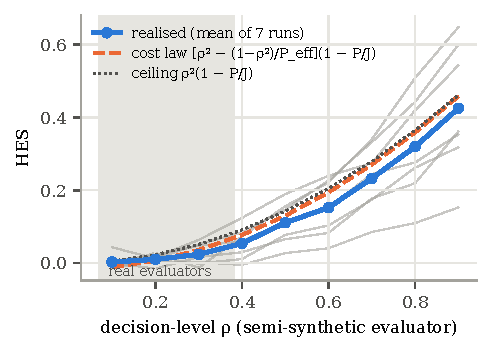
\includegraphics[width=\columnwidth]{figures/F3_rho_dial.pdf}
\caption{Realised HES of semi-synthetic evaluators with a set decision-level $\rho$ (grey: individual runs) against the
cost law (\ref{eq:law}) and its oracle-$\lambda$ ceiling. Shaded: the range of the real evaluators.}\label{fig:dial}
\end{figure}

\paragraph{The estimation tax on real metrics.} Replacing the pilot-fitted coefficient by the population-optimal one
isolates the tax. Over the 31 metric variants it is 4.3 [3.5, 5.2] points on en$\to$de and 2.5 [2.0, 3.1] on zh$\to$en
(metric-level bootstrap; H9). For the five metrics with the largest $\rho^2$ (0.11--0.14 on en$\to$de as $(\bar\rho)^2$, 0.11--0.15 as mean $\rho^2$, within the 0.09--0.15 PPSR reports),
the realised saving over uniform sampling is between $-3\%$ and $+6\%$ (en$\to$de) and $-6\%$ and $+1\%$ (zh$\to$en), below the correlation-based saving in every cell. H10 held under the locked $(\bar\rho)^2$ definition and
was unchanged in a post-lock robustness check with PPSR's mean of squared correlations $\overline{\rho^2}$. With the oracle coefficient the same en$\to$de metrics reach 6--12\% on the decision-aware
design: the asymptotic saving is not wrong, it is what an auditor who already knew $\lambda$ would obtain.

\paragraph{Is the tax an artefact of freezing $\lambda$?} Largely, yes. Standard PPI++ fits $\lambda$ on all labelled
items. We re-ran the eight strongest metric variants per language pair, COMET-22 and the two GEMBA judges with the
coefficient refitted by least squares on the pilot and every post-pilot label, and cross-fitted over two folds
(exploratory, Appendix~\ref{app:robust}). Mean HES on the weighted design rises from $+0.4\%$ (pilot coefficient) to
$+6.8\%$ with refitting and $+1.6\%$ with cross-fitting on en$\to$de, against $+6.7\%$ for the oracle coefficient; on
zh$\to$en from $-0.4\%$ to $+2.0\%$ and $+1.1\%$, against $+1.3\%$; on the six chat pairs from $+1.1\%$ to $+2.3\%$ and $+1.5\%$, against $+2.1\%$. Under boundary stress the refitted certificate's largest
type-I error was 0.05 and no cell was significantly above $\alpha$, although its variance estimate ignores the
coefficient's estimation error. The tax is therefore the price of committing to the coefficient before the audit (for
instance to plan the budget), not a property of the evaluator. The evaluators remain modest even without it: on the
best fixed judge-free base, the mean over the eleven with refitting is 6.9\% and 6.7\% (en$\to$de, $\eps=0.01, 0.02$) and
4.8\% and $-0.3\%$ (zh$\to$en), below the design's 15.9\%, 9.0\%, 8.4\% and 8.5\%; the best of the eleven, chosen post hoc,
reaches 10.6\%, 12.1\%, 15.4\% and 1.0\%.

\paragraph{Pilot size trades tax for fixed cost.} Equation~(\ref{eq:law}) predicts that a larger pilot lowers the tax
$(1-\rho^2)/P_{\mathrm{eff}}$ but raises the fixed cost $P$. Both effects appear. Doubling the MT pilot to 100 segments
shrinks the losses of the weak LLM judges (Mistral-7B on en$\to$de at $\eps=0.01$: $-7.1\%\to-0.9\%$) without making any
LLM judge save more than 4\%; for the semi-synthetic evaluator with $\rho=0.9$ on en$\to$de, the same doubling halves the
saving (mean over $\eps$, 32\%$\to$15\%; 46\%$\to$27\% at $\eps=0.01$) because the pilot becomes most of the cost. With pilots of 25--100 items a $\rho\approx0.2$ evaluator does not pay; by (\ref{eq:law}) its saving stays below
$\rho^2(1-P/J)\approx4\%$ even with a much larger pilot.

\section{Chat: close pairs and presentation order}\label{sec:arena}
For the six close Arena pairs the pairwise judges reach (pilot-median) decision-level $\rho$ between $-0.01$ and 0.29, and the length heuristic 0.07--0.21. The best judge saves at least
5\% with an interval above zero in two pairs (Figure~\ref{fig:arena}a; H6 required three). Position bias explains part of
the low $\rho$: judging one presentation order only gives $\rho$ of 0.19 (Qwen3-8B) and 0.12 (Mistral-7B); averaging both
orders raises it to 0.25 and 0.16 and turns Mistral's realised saving from $-1$ to $-2\%$ into $+0.5\%$ (mean over
$\eps\in\{0.02,0.05,0.1\}$). Averaging two judgments is also an ensemble, so the gain cannot be attributed to de-biasing alone. As with a
mean bias toward a policy in retrieval, the bias itself is corrected by the human labels; the noise it adds lowers $\rho$
and costs efficiency.

\begin{figure*}[t]\centering
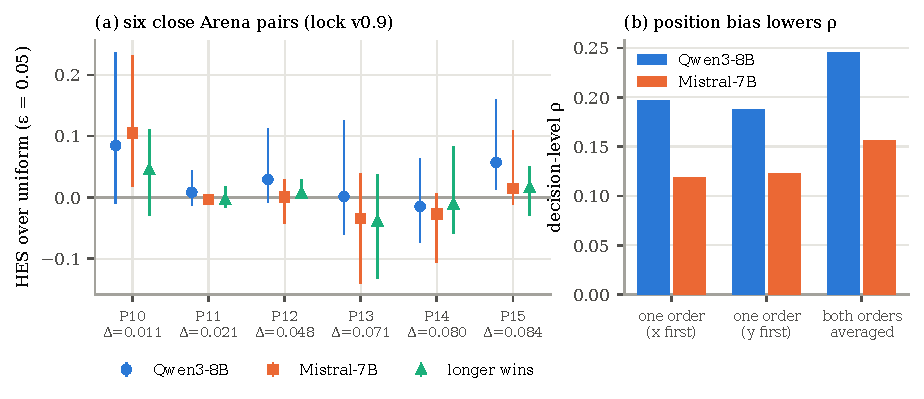
\includegraphics[width=\textwidth]{figures/F4_arena.pdf}
\caption{(a) HES over uniform sampling of three evaluators on six close LMArena pairs ($\Delta$: human win-rate gap;
pilot 50, $\eps=0.05$; 95\% intervals). (b) Decision-level $\rho$ with one presentation order and with both orders averaged.}\label{fig:arena}
\end{figure*}

\section{Pre-registered outcomes and validity}\label{sec:prereg}
Table~\ref{tab:prereg} lists every pre-registered hypothesis. The design-dominance and estimation-tax hypotheses held;
H2, H5 and H6 did not, and H4 held only in MT. H2 predicted that evaluator value measured over uniform sampling would be inflated by at least 5 points
relative to the best design; with the open judges the value was near zero on both baselines, so there was nothing to
inflate. H5 predicted that selecting an evaluator by its pilot-predicted cost would beat selecting by pilot accuracy; it
did worse in both domains (excess cost over the best fixed arm 3.2\% vs.\ 2.3\% in MT, 2.8\% vs.\ 1.7\% in chat): when
every candidate is near break-even, a 50-item pilot cannot resolve their differences, which by (\ref{eq:law}) are a few
points. H4 (pilot predicts relative design cost) held in MT (median correlation 0.82) but not in chat (0.37), where
the only lever is the evaluator and the cost ratios differ by little.

\begin{table}[t]\centering\footnotesize\setlength{\tabcolsep}{2.5pt}
\resizebox{\columnwidth}{!}{\begin{tabular}{llc}\toprule
& Hypothesis & Outcome\\\midrule
H1 & design saving $>$ best open judge (MT) & 4/4\\
H2 & inflation $\ge$ 0.05 (MT) & \textbf{0/4}\\
H3 & HES tracks $\rho$ $>$ accuracy$^a$ & held (MT weak)\\
H4 & pilot predicts cost ($r\ge.8$) & MT; \textbf{chat no}\\
H5 & pilot selector beats accuracy & \textbf{no (both)}\\
H6 & chat HES $\ge$5\% in $\ge$3/6 & \textbf{2/6}\\
H8 & design $\ge$ best of 31 variants$^b$ & 4/4\\
H9 & estimation tax $>0$ & both pairs\\
H10 & realised HES $<\rho^2$ (top 5)$^c$ & all cells\\
H11 & HES tracks $\rho$ $>$ system $r$ & both\\\bottomrule
\end{tabular}}
\caption{Pre-registered hypotheses (locks v0.8, v0.9, v1.1). $^a$on two-system menus. $^b$with the locked pilot-fixed
coefficient; with a refitted coefficient the post-hoc best of the eleven strongest exceeds the design in 2/4 cells.
$^c$largely implied by the dilution factor $1-P/J$. H7 and H2$'$ belong to the frontier-judge lock v1.0, not yet run.}\label{tab:prereg}
\end{table}

\paragraph{Validity.} Over all locked cells the observed wrong-certificate rate is at most 0.070 (Clopper--Pearson upper
limit 0.105). Under boundary stress (the runner-up as candidate, $\eps$ at 0.9 times its regret) the largest observed
type-I error among 882 chat cells is 0.143 at nominal 0.10; an exact binomial test per cell finds no cell significantly
above $\alpha$ after Bonferroni correction (0.5\% of cells at $p<0.05$), and a Student-$t$ bound changes the maximum to
0.140. These are Monte-Carlo checks of an asymptotic bound, not finite-sample guarantees.

\section{Related work}
\paragraph{Judges and metrics as system rankers.} JuStRank \citep{gera2025justrank} and \citet{gao2025reeval} show that
instance-level accuracy does not determine system-ranking quality and that ranking degrades for close systems;
\citet{zhang2026utility} separate judgment quality from downstream utility. We follow quality one level further, to the
human labels a close decision requires.
\paragraph{Prediction-powered evaluation.} PPI and PPI++ \citep{angelopoulos2023ppi,angelopoulos2023ppipp}, active
inference \citep{zrnic2024active}, AutoEval and prediction-powered ranking on Chatbot Arena
\citep{boyeau2024autoeval,chatzi2024ppr}, efficient noisy-judge inference \citep{chen2026noisy}, PRECISE for ranking
metrics \citep{divekar2026precise}, and the bound of \citet{dorner2025limits} that an evaluator no better than the
evaluated model saves at most half the labels. Closest to us, \citet{gao2026ppsr} rank WMT metrics by the annotation they
save under prediction-powered evaluation (PPSR, the mean squared correlation of paired differences), with uniform
labelling and the coefficient estimated on the evaluation labels. We take PPSR's quantity as the starting point and
measure what remains of it under a decision-aware design and a pilot-fixed coefficient.
\paragraph{Annotation design.} Choosing which items humans label has long been studied for model comparison
\citep{sawade2012active}, active testing \citep{kossen2021active} and IR test collections
\citep{sakai2016topic,li2017active}, and within prediction-powered inference by cross-prediction
\citep{zrnic2024cross} and stratification \citep{fisch2024stratified}. Our judge-free designs are simple instances
(skipping known zeros, deduplication, proxy-weighted sampling); the point is to credit them before the evaluator.

\section{Conclusion}
For a close system decision, an automatic evaluator's value is set by the correlation of the differences the decision
depends on, not by its system-level agreement, and it is diluted by the fixed cost of the pilot and by what a judge-free
design already obtains. Under these conditions the strongest WMT22 metric variants and open LLM judges save on average
between nothing and about 7\% of human labels, even with the correction refitted on all labels, while organising the
human annotation itself, mostly by not paying twice for identical outputs, saves 8--16\% in MT. Committing to the
correction before the audit costs a few points more. Reporting the decision-level correlation next to system-level
agreement, and crediting the annotation design before the evaluator, would make claims of evaluator savings comparable
to what an audit actually obtains.

\section*{Limitations}
The menus are built from full human labels to be deliberately hard; easier decisions leave less to save for any method.
The certificate uses a normal bound whose calibration we checked by simulation, not proved. MT savings are computed on
the MQM-rated subsets of WMT22 (two language pairs), chat on six pairs from a 2023 Arena release, retrieval on
re-analysed audits of an earlier study with two judges. The cost law is a first-order approximation; it describes
controlled variation of $\rho$ and bounds, but does not predict cell by cell, the savings of real evaluators. Frontier
LLM judges are not evaluated here; their pre-registration is committed. HES depends on the pilot size, and larger pilots
lower the estimation tax while raising the fixed cost (\S\ref{sec:law}). The results should not be read as showing
that automatic evaluators are useless: they concern close decisions, small human pilots and evaluators with
decision-level $\rho\le0.38$; by the cost law, an evaluator with $\rho\approx0.8$ would save about a third of the labels.

\bibliography{refs}

\appendix
\section{Derivation of the cost approximation}\label{app:law}
Write $D$ for the paired difference of an informative item, $\sigma^2=\mathrm{Var}(D)$, and $\hat D$ for the evaluator's
prediction with $\mathrm{Corr}(D,\hat D)=\rho$. For a fixed coefficient $\lambda$ the residual $R=D-\lambda\hat D$ has
variance $\sigma^2-2\lambda\rho\sigma\hat\sigma+\lambda^2\hat\sigma^2$, minimised at $\lambda^\star=\rho\sigma/\hat\sigma$ to
$\sigma^2(1-\rho^2)$ \citep{angelopoulos2023ppipp}. With $\hat\lambda$ the least-squares coefficient from
$P_{\mathrm{eff}}$ pilot items, independent of the post-pilot sample, and a homoskedastic residual ($\mathrm{E}[R^2\mid\hat D]=\sigma^2(1-\rho^2)$), $\mathrm{E}[(\hat\lambda-\lambda^\star)^2]\approx
\sigma^2(1-\rho^2)/(P_{\mathrm{eff}}\hat\sigma^2)$, so the expected residual variance is
$\sigma^2(1-\rho^2)(1+1/P_{\mathrm{eff}})$ \citep[\S7]{cochran1977}. Under the normal fixed-budget approximation the
post-pilot labels needed to bring $z\sqrt{v/L}$ below the slack scale with the variance factor, so
$L\approx L_0(1-\rho^2)(1+1/P_{\mathrm{eff}})$ and $1-L/L_0\approx\rho^2-(1-\rho^2)/P_{\mathrm{eff}}$ to first order in
$1/P_{\mathrm{eff}}$. With the pilot cost $P$ common to both arms, $\HES=1-(P+L)/(P+L_0)=(1-L/L_0)(1-P/J_0)$. Clipping
$\lambda$ at zero bounds the loss of an evaluator with $\rho\le0$ by the variance of $\hat\lambda$ only; zero-difference
items reduce $P_{\mathrm{eff}}$ below $P$, which is why MT, with about half its paired differences zero, pays more tax.
In general, $\mathrm{Var}(\hat\lambda)\approx\mathrm{E}[(\hat D-\mathrm{E}\hat D)^2R^2]/(P_{\mathrm{eff}}\hat\sigma^4)$ (sandwich form), which reduces to the expression above under homoskedasticity; heavy-tailed or heteroskedastic residuals, as with sparse MQM differences, raise the tax.

\section{Robustness of the estimation tax}\label{app:robust}
Mean HES over the evaluators of each set, over their own judge-free base, by how the coefficient is set ($\Jt$; MT:
eight strongest metric variants per language pair, COMET-22, Qwen3-8B, Mistral-7B; chat: Qwen3-8B, Mistral-7B,
longer). Pilot: fitted on the pilot and frozen (the paper's estimator); refit: refitted by unweighted least squares on the pilot
and every post-pilot label; xfit: cross-fitted over two folds; HT: the same with $1/\pi$-weighted least squares;
oracle: population-optimal.

\begin{center}\footnotesize\resizebox{\columnwidth}{!}{\begin{tabular}{llrrrrrr}\toprule
Cell & base & pilot & refit & xfit & refit$_{\mathrm{HT}}$ & xfit$_{\mathrm{HT}}$ & oracle\\\midrule
MT en$\to$de & weighted & 0.4 & 6.8 & 1.6 & 10.0 & $-1.3$ & 6.7\\
MT en$\to$de & dedup & 0.8 & 7.2 & 1.7 & 12.4 & $-1.3$ & --\\
MT zh$\to$en & weighted & $-0.4$ & 2.0 & 1.1 & 2.0 & 1.1 & 1.3\\
MT zh$\to$en & dedup & $-1.8$ & 2.3 & 1.9 & 2.5 & 2.3 & --\\
Chat (6 pairs) & uniform & 1.1 & 2.3 & 1.5 & 2.3 & 0.9 & 2.1\\\bottomrule
\end{tabular}}\end{center}
Values in \%, averaged over $\eps$. With $J_{80}$ in place of $\Jt$ the MT values are 0.1--1.2 (pilot), 2.2--4.9 (refit),
1.5--2.8 (xfit), 2.1--4.4 (refit$_{\mathrm{HT}}$), 0.7--2.9 (xfit$_{\mathrm{HT}}$) and 1.9--2.5 (oracle); $J_{80}$ is often near
the largest budget, so these are less reliable. Under boundary stress the largest type-I errors on en$\to$de were 0.04 (pilot), 0.047 (refit),
0.043 (xfit), 0.07 (refit$_{\mathrm{HT}}$), 0.05 (xfit$_{\mathrm{HT}}$) and 0.06 (human-only); no cell was significantly
above $\alpha$. Evaluator-driven allocation (sampling by the pilot-estimated residual
variance, as in active inference) reduced $\Jt$ relative to the weighted design with the same evaluator by $-1.6\%$ to
$+1.7\%$ on average over the 31 metric variants (individual cells $-11\%$ to $+19\%$).

\section{Pre-registration record}\label{app:prereg}
Lock v0.8 (MT, chat; hypotheses H1--H5 and validity) was committed before any LLM or COMET judgment was joined with a
human label; the human-only MT designs and chrF had been examined in development and are reported as such. Two
deviations followed (a type fix and an accounting fix charging one Arena vote per battle). Lock v0.9 replaced the v0.8
chat decision, whose pairs had win-rate gaps of 0.10--0.56 and were certified by every design right after the pilot, by
the six closest pairs; no judge output existed for these battles. Lock v1.1 fixed the 31-metric test (H8--H11) before
any of its savings were computed; H10 as locked uses $(\bar\rho)^2$ and is reported with PPSR's mean of squared
correlations as a post-lock robustness check, and H9's interval is a metric-level bootstrap. Lock v1.0 (frontier
judges) is committed with its exported inputs and scoring rule and has not been run. Analyses not listed in a lock
(three-level anatomy, oracle-$\lambda$ tax for open judges, presentation order, semi-synthetic $\rho$) are exploratory.

\end{document}
